\section{Method}

We introduce a memory intervention architecture for long-horizon language agents.
The goal is to maintain decision-relevant execution state over a multi-step
trajectory and selectively reactivate that state when it is likely to affect the
action agent's next decision. Our method leaves the action agent unchanged and
adds a separate memory agent that observes the trajectory, updates a structured
memory bank, and decides whether to inject a concise reminder into the action
agent's context. Figure~\ref{fig:method_overview} summarizes the architecture:
the left panel shows how the memory agent is integrated with the action agent
in the run loop, and the right panel zooms into the memory agent's two-phase
internal workflow.


\begin{figure*}[t]
\centering
\begin{subfigure}[t]{0.48\textwidth}
\centering
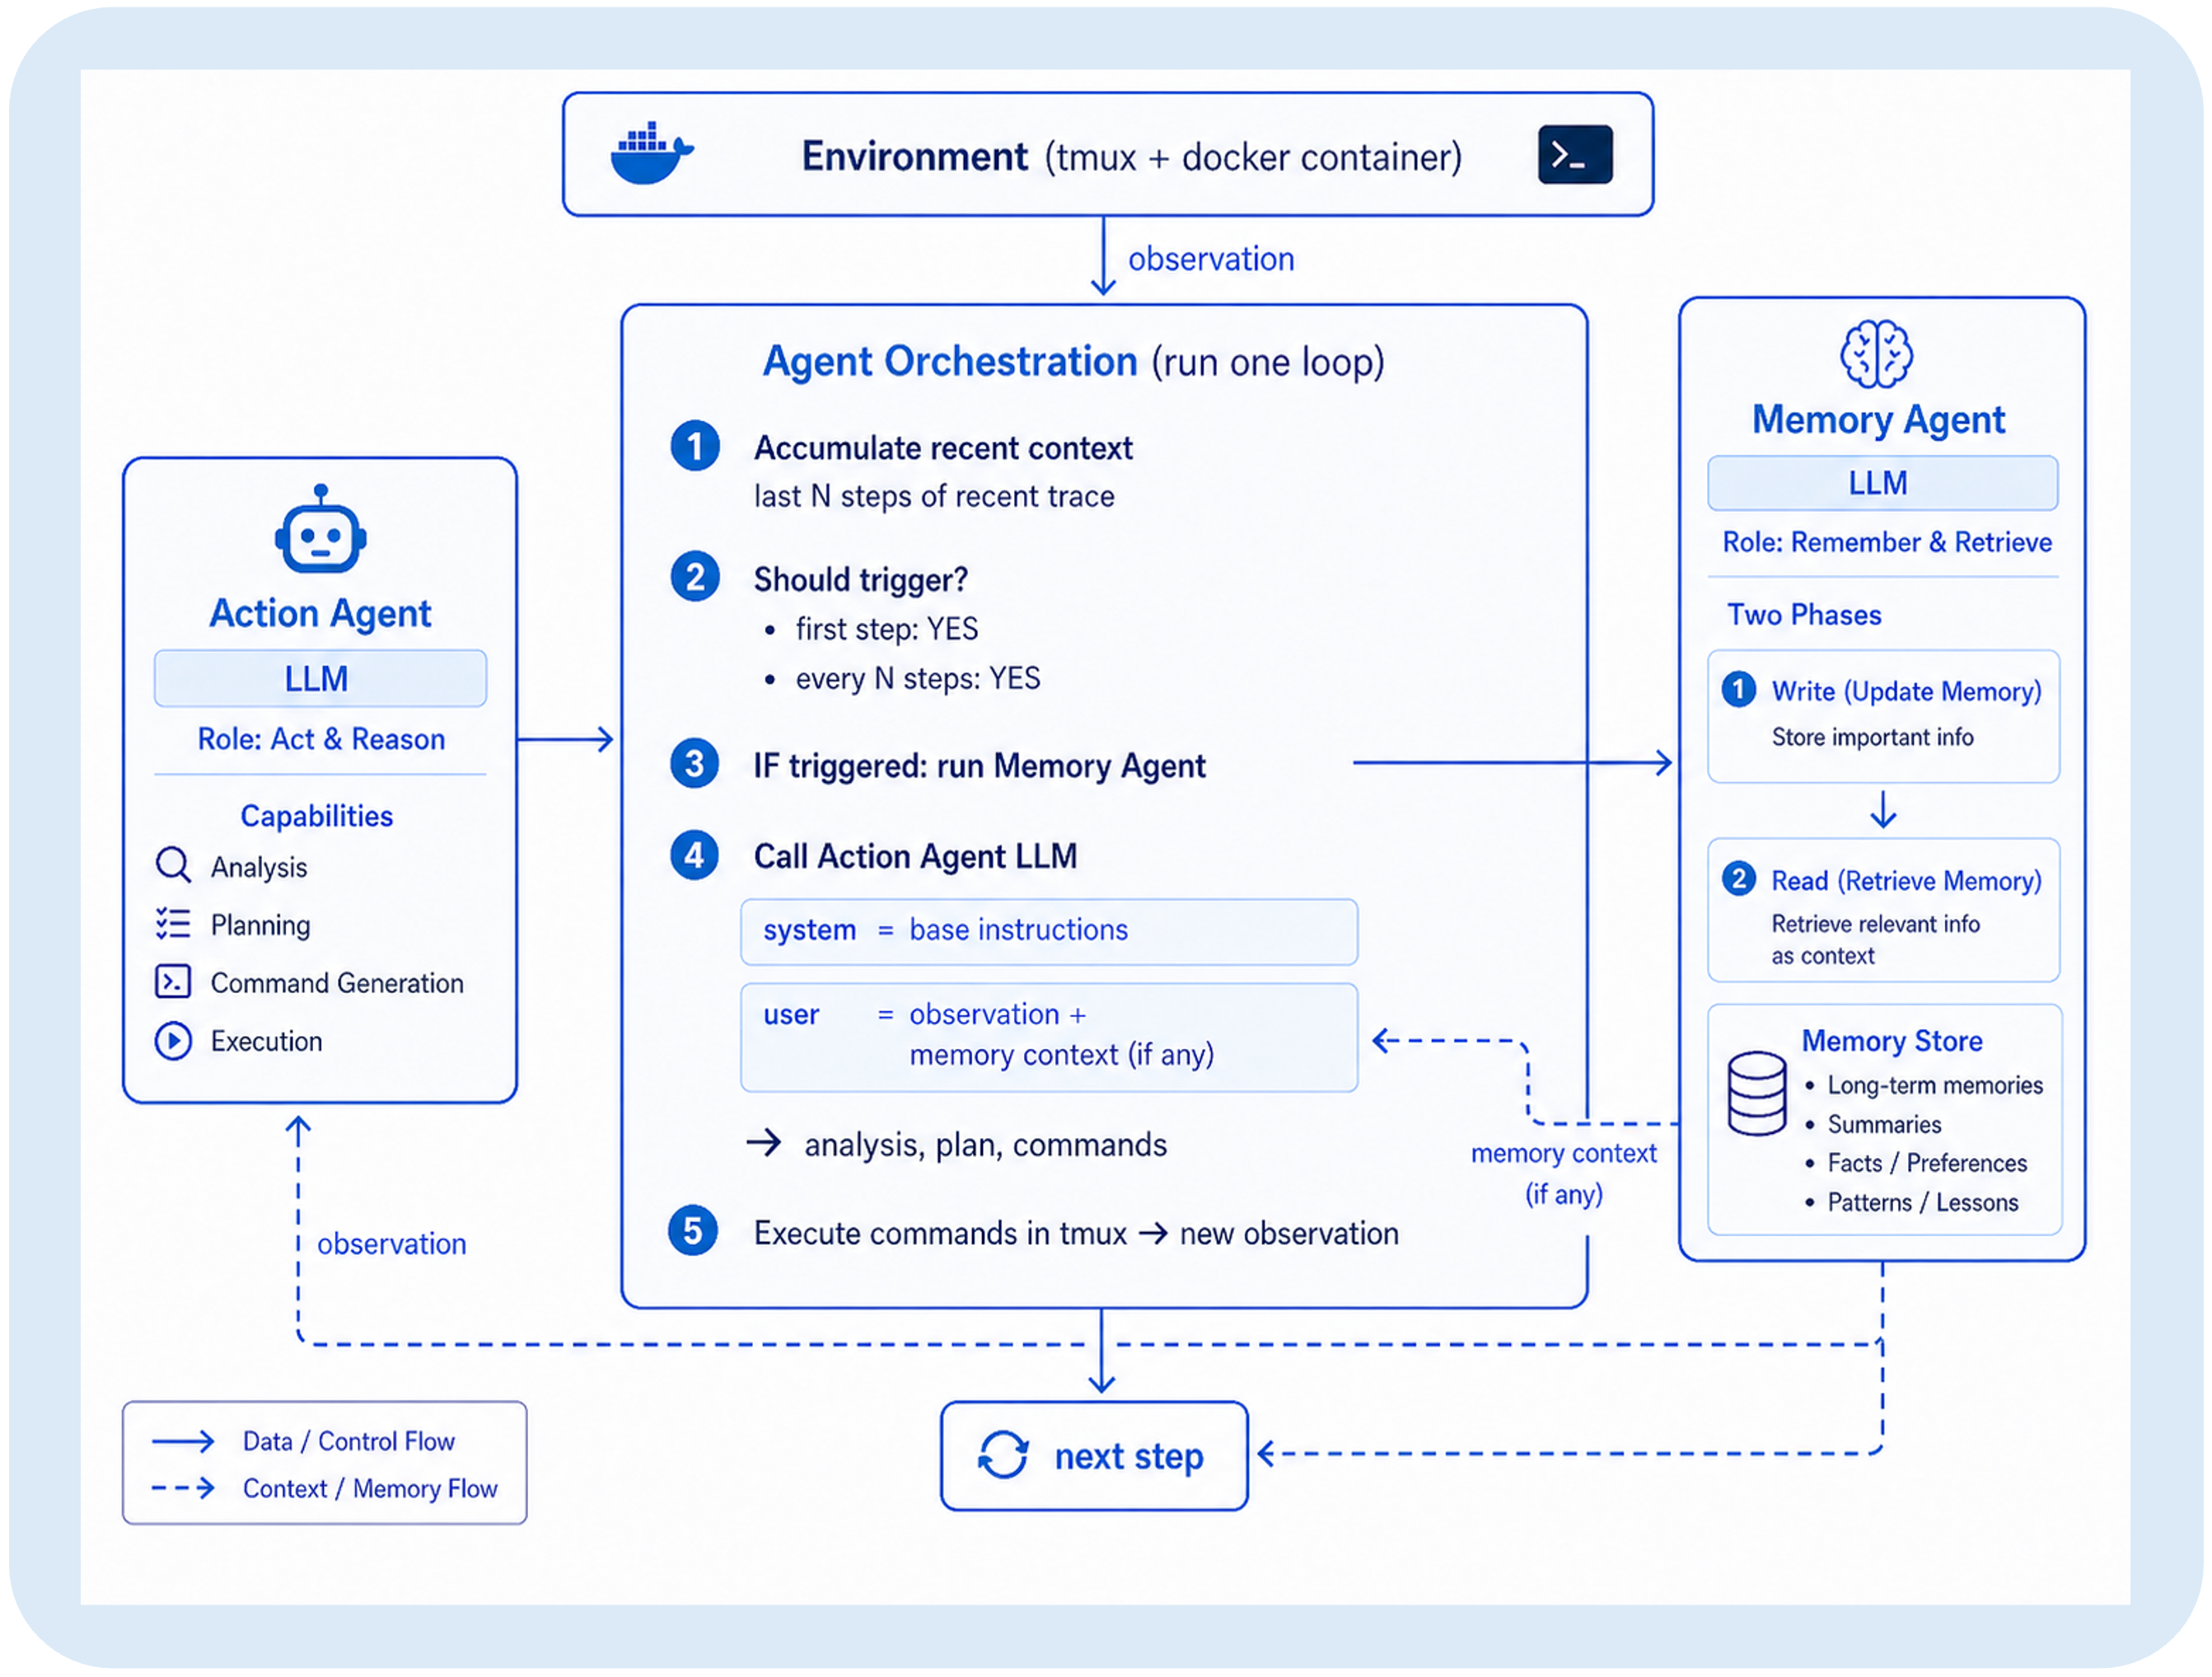
\includegraphics[width=\linewidth]{assets/Picture2.png}
\caption{System integration. The action agent (left) interacts with the
environment; the memory agent (right) runs alongside, observing a sliding
window of recent steps and the current memory store. At every $N$ steps the
memory agent is invoked to update the bank and optionally inject a context
reminder into the next action-agent call.}
\label{fig:method_system}
\end{subfigure}\hfill
\begin{subfigure}[t]{0.48\textwidth}
\centering
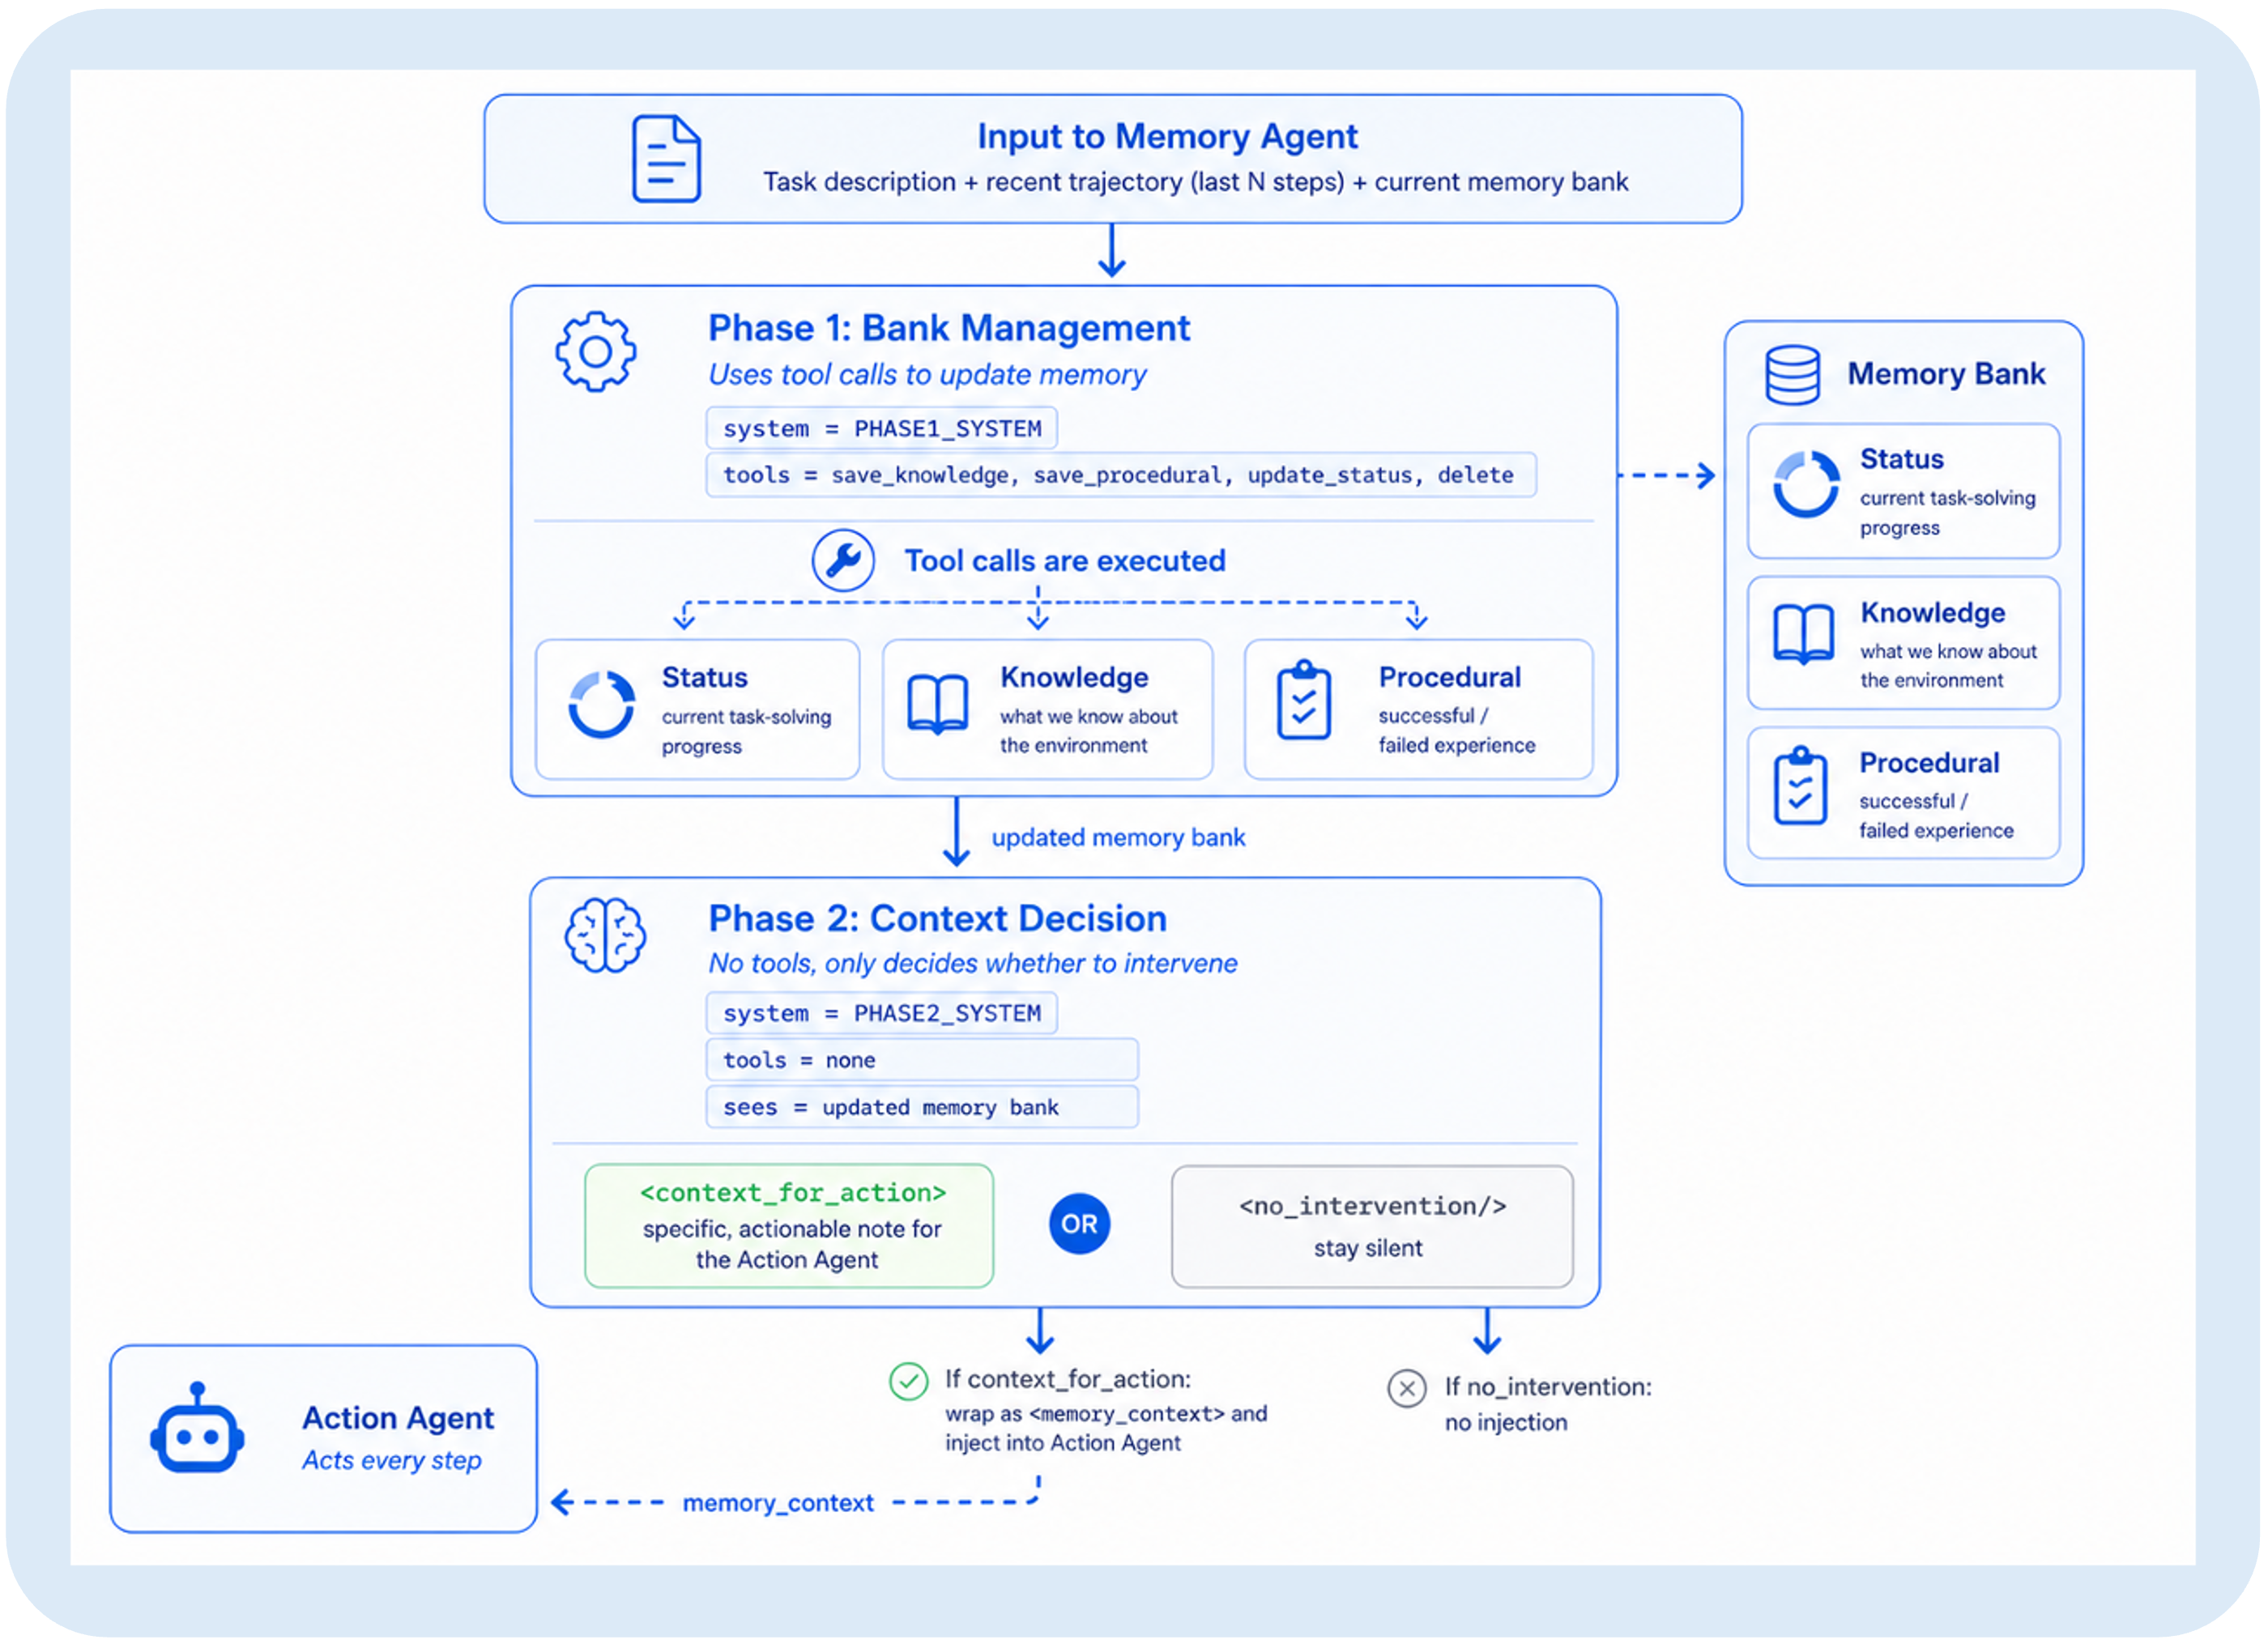
\includegraphics[width=\linewidth]{assets/Picture1.png}
\caption{Memory agent internals. Phase~1 manages the memory bank
(\emph{status}, \emph{knowledge}, \emph{procedural} entries) through tool
calls. Phase~2 reads the updated bank and either emits a
\texttt{<context\_for\_action>} reminder or \texttt{<no\_intervention/>}.}
\label{fig:method_memory_agent}
\end{subfigure}
\caption{Overview of the memory-intervention architecture. (a) The memory agent
runs as a separate process beside an unmodified action agent. (b) Within each
memory step, a two-phase workflow first updates the structured memory bank,
then decides whether any remembered state should enter the action agent's next
decision.}
\label{fig:method_overview}
\end{figure*}

\subsection{Problem Setup}


We consider an action agent interacting with an environment over a trajectory
$\tau = (o_1, a_1, o_2, a_2, \ldots, o_T)$, where $o_t$ is the environment
observation at step $t$ and $a_t$ is the action produced by the agent. The
agent is given a task description $x$ and samples
$a_t \sim \pi_A(a_t \mid x, \tau_{<t})$, where $\pi_A$ is the action policy
implemented by an LLM and tool-use scaffold. In long-horizon settings, the
context the scaffold actually exposes to $\pi_A$ may be truncated, summarized,
or otherwise filtered, so not every piece of trajectory information remains
available at each step.

In long-horizon tasks, the full trajectory may contain many pieces of information
that should continue to influence future actions even when they are no longer
salient in the action-agent context: task requirements, environment facts, previous attempts,
failure diagnoses, intermediate discoveries, and open subgoals. We refer to this
information as \emph{execution state}. Our objective is to maintain execution
state separately from the action context and decide when it should be reintroduced
into the action loop.

We augment the action agent with a memory agent $\pi_M$. The memory agent is
invoked at the first step and then at a fixed interval. At each memory timestep
$t$, it observes the task description, a recent trajectory window
$w_t = \mathcal{W}_k(\tau_{<t}, o_t)$, and the current memory bank $B_{t-1}$.
It first updates the bank and then decides whether to emit an intervention:
\[
\begin{aligned}
B_t &\sim \pi_M^{\mathrm{edit}}(\cdot \mid x, w_t, B_{t-1}), \\
i_t &\sim \pi_M^{\mathrm{intervene}}(\cdot \mid x, w_t, B_t),
\end{aligned}
\]
where $i_t \in \{\varnothing, \text{text reminder}\}$. A non-null intervention
is injected into the next action-agent call as transient memory context;
otherwise the action agent proceeds without additional memory context.

This formulation treats memory as a policy over interventions. The memory agent
must decide not only what execution state to retain, but also when remembered
state is useful enough to enter the action loop.

\subsection{Memory Bank}

The memory bank is a compact, structured representation of execution state. It
contains three components:
\[
B_t = (s_t, K_t, P_t),
\]
where $s_t$ is a private status field, $K_t$ is a set of knowledge memories, and
$P_t$ is a set of procedural memories.

The \textbf{status} field tracks the memory agent's private view of progress,
open issues, and unresolved risks. It is never shown to the action agent. This
allows the memory agent to maintain a working model of the task without
polluting the action agent's context.

The \textbf{knowledge} memory stores relatively stable facts that are expected
to remain true during the task, such as task requirements, environment
properties, file paths, configuration details, user- or tool-verified facts, and
evaluation-relevant observations. These entries capture what the agent has
learned about the task or environment.

The \textbf{procedural} memory stores attempts and outcomes, such as commands
that failed, fixes that succeeded, hypotheses that were ruled out, diagnostic
signals, or empirical improvements. These entries capture what the agent has
tried and what happened, so that later decisions can avoid repeated failures or
reuse successful evidence.

Each memory entry consists of a short identifier, natural-language content, and
metadata such as creation time and access statistics. Identifiers allow the
memory agent to update or delete stale entries explicitly. In practice, entries
are written in a compact tagged format, such as environment facts, paths, task
facts, bugs, and performance observations. This structure encourages the memory
agent to distinguish constraints from procedural evidence.


\subsection{Two-Phase Memory Agent}

At each memory step, the memory agent runs two phases: memory bank management
and proactive intervention.

\paragraph{Phase 1: Memory management.}
In the first phase, the memory agent manages the memory bank by returning a list
of predefined tool calls. It does not directly rewrite the memory bank. Given the
task description, the recent trajectory window, and the current bank, the memory
agent may call memory\_update\_status, memory\_save\_knowledge,
memory\_save\_procedural, and memory\_delete zero or more times. The system
executes the returned calls in order and treats the resulting bank as the updated
memory bank. If the memory agent returns no tool call, the bank is left
unchanged.

The four calls correspond to the three memory components and deletion.
memory\_update\_status updates the memory agent's private progress tracking,
which is used only by the memory agent and is not shown to the action agent.
memory\_save\_knowledge saves important facts to the knowledge bank, including
task requirements, environment facts, file paths, API details, and key
constraints from the task description. memory\_save\_procedural records
debugging experience, failed approaches, solutions, error patterns, successful
fixes, and performance observations. memory\_delete removes an outdated or
incorrect memory entry by its identifier.

This tool-call interface makes memory management explicit and constrained: the
Phase~1 output is a sequence of bank edits, not a free-form summary of the
trajectory. It lets the memory agent externalize execution state such as
unsatisfied requirements, verified environment facts, failed commands, and
successful fixes while keeping the bank structured across long trajectories.

\paragraph{Phase 2: Intervention selection and transient injection.}
Conditioned on the updated memory bank and the recent trajectory, the memory
agent selects an intervention action for the next action-agent decision. This
phase does not modify the memory bank. Instead, it decides whether any retained
execution state should be reactivated, and if so, how it should be expressed as
a targeted reminder. Formally, the intervention action is either a reminder
$r_t$ or a null intervention $\varnothing$.

If the memory agent emits a reminder, the system supplies $r_t$ to the next
action-agent call as a separate transient memory context. The action agent's
base instructions, tools, and decoding procedure are unchanged; the only change
is the optional memory context provided at call time. If the memory agent selects
the null intervention, the action-agent context is left unchanged.

The null intervention is an explicit action. The memory agent is encouraged to
intervene only when a remembered item is likely to affect the next action-agent
decision. Useful interventions include reminders of requirements that are about
to be violated, environment facts that explain the current observation, previous
attempts that should not be repeated, diagnoses that remain relevant, or open
subgoals that are being neglected. The memory agent is discouraged from giving
broad strategic advice, restating information already visible in the current
observation, or taking over the action agent's planning. Thus, intervention
timing is part of the memory policy rather than a consequence of every memory
update.

\subsection{Triggering the Memory Agent}

The memory agent is invoked according to a trigger function $g(t)$. In our main
implementation, it runs at the first step and then at a fixed interval. This
simple schedule lets the memory agent track the trajectory closely and decide
whether to remain silent or intervene. More selective triggers are possible, such
as invoking memory only after tool errors, failed tests, repeated commands, or
large context shifts, but we use a fixed interval to isolate the effect of the
memory intervention policy itself.


\subsection{Learning Memory Intervention Policies}
The memory-intervention architecture does not require training a new model. In
our main instantiation, the memory agent can be implemented as a prompted model
that follows the two-phase interface described above. However, prompted memory
agents are not necessarily the most practical deployment setting: they add
additional inference cost, and their intervention decisions may be imperfectly
calibrated. We therefore treat training an open-weight memory agent as an early
exploration of whether the same intervention policy can be learned rather than
only prompted.

We train only the memory agent while keeping the action agent fixed. Supervised
fine-tuning distills trajectories from a prompted memory agent, teaching the
model to perform memory-bank operations and to choose between a targeted reminder
and a null intervention. This stage mainly teaches the interface and basic
discipline of memory management: compact writing, updating stale state, and
avoiding unnecessary reminders.

Because imitation alone does not optimize the downstream effect of memory
interventions, we further calibrate the memory agent with reinforcement learning.
The goal is not to maximize memory usage, but to improve the intervention policy:
the trained model should learn when remembered execution state is likely to help
the next action decision, and when silence is preferable. We view this training
study as preliminary evidence that memory intervention can be distilled into an
open-weight policy; the architecture itself remains independent of this training
procedure.
% \begin{comment}
% The key distinction between our approach and ordinary summarization is that the
% memory agent does not merely compress the trajectory. A summarizer asks what
% information should be retained. Our memory agent asks a stronger control
% question: given the current state of the task, should any remembered execution
% state become active in the action agent's next decision?

% This distinction matters because long-horizon tasks vary substantially in their
% failure modes. In some tasks, the useful memory is a hard requirement from the
% initial instruction; in others, it is an environment fact, a previous failed
% command, a bug diagnosis, or an unfinished subgoal. A fixed summarization policy
% cannot know whether a memory should interrupt the next action. Our method learns
% this intervention policy explicitly.
% \end{comment}

